\documentclass[a4paper,graphics,11pt]{article}

\usepackage[utf8]{inputenc}
\usepackage[T1]{fontenc}
\usepackage{lmodern}
\usepackage[ngerman]{babel}
\usepackage{amsmath, tabu}
\usepackage{amsthm}
\usepackage{amssymb}
\usepackage{algorithm}
\usepackage{algpseudocode}
\usepackage{mathtools}
\usepackage{setspace}
\usepackage{graphicx,color,curves,epsf,float,rotating}

\floatname{algorithm}{Algorithmus}

\newcommand\norm[1]{\left\lVert#1\right\rVert}
\newcommand\abs[1]{\left\vert#1\right\vert}

\newcommand\aufgabe[1]{\subsection*{Aufgabe #1}}
\newcommand\aufgabenteil[1]{\subsubsection*{#1}}



\pagestyle{empty}
\begin{document}
\noindent WS 2016/17        \hfill Simon Kaiser, 354692 \\
\null                                     \hfill Philipp Hochmann, 356148 \\
\null                                     \hfill Felix Kiunke, 357322 \\
\null                                     \hfill Giacomo Klingen, 356778 \\
\null                                     \hfill Daniel Schleiz, 356092 \\

\begin{center}
\Large \textsc{Softwaretechnik} \\   % Fach
\large Aufgabenblatt 3                        % Nummer das Blattes, nicht vergessen zu ändern!
\end{center}
\begin{center}
\rule[0.5ex]{\textwidth}{0.6pt}\vspace*{-\baselineskip}\vspace{3.2pt}
\rule[0.5ex]{\textwidth}{1.6pt}\\
\end{center}

\DeclareGraphicsExtensions{.jpg}
%%%%%%%%%%%%%%%%%%%%%%%%%%%%%%%%%%%%%%
%
%   Ab hier kommt der Text
%   Neue Aufgabe mit \aufgabe{}
%   Aufgabenteil mit \aufgabenteil{}
% 
%%%%%%%%%%%%%%%%%%%%%%%%%%%%%%%%%%%%%%

\aufgabe{3.1}

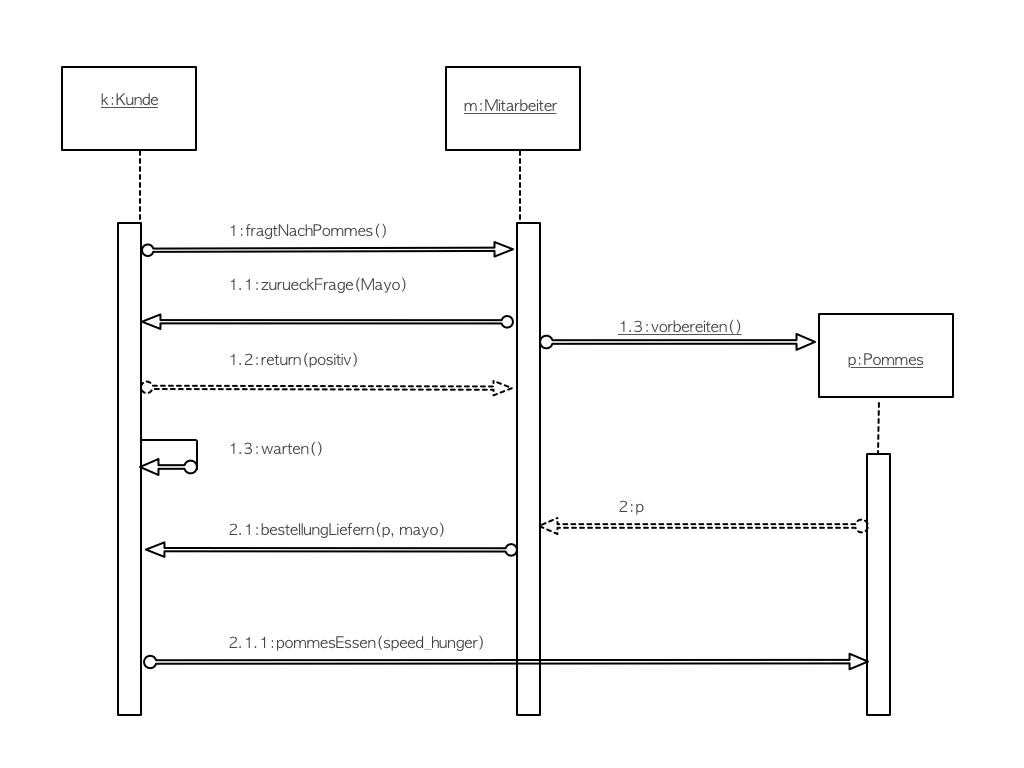
\includegraphics[width=1\textwidth]{SWT31}

\aufgabe{3.2}
\aufgabenteil{a}
TBC
\aufgabenteil{b}
TBC
\aufgabe{3.3}
TBC as well
\end{document}
% Nummer des Blattes angepasst?
